% ACL Rolling Review long paper: 8 pages of content. Limitations, Ethical Considerations,
% references and appendices do not count. Official *ACL style files, unmodified; the preamble
% matches ../../mechanism-population-dynamics/paper-acl-v3/main.tex.
% Figures and numbers: ../scripts/paper_figures_v2.py (computed from ../results).
\documentclass[11pt]{article}

\usepackage[review]{acl}
\usepackage{times}
\usepackage{latexsym}
\usepackage[T1]{fontenc}
\usepackage[utf8]{inputenc}
\usepackage{microtype}
\usepackage{inconsolata}
\usepackage{graphicx}
\usepackage{booktabs}
\usepackage{makecell}
\usepackage{amsmath,amssymb}
\usepackage{xcolor}
\usepackage{adjustbox}
\usepackage[inline]{enumitem}
\usepackage{tikz}
\usetikzlibrary{positioning,arrows.meta,calc,fit,backgrounds}

\definecolor{srcA}{HTML}{2F6DB3}
\definecolor{srcB}{HTML}{E08A2C}
\definecolor{blk}{HTML}{C4473D}
\definecolor{nameC}{HTML}{3C9A64}
\newcommand{\ns}[1]{\textcolor{gray}{#1}}
\newcommand{\lw}[1]{\textit{#1}}
\newcommand{\nmodels}{eight}
\makeatletter\newcommand{\rows}[1]{\@@input #1 }\makeatother
\newcommand{\ci}[2]{{\scriptsize\,(#1, #2)}}

\title{Whose Rule Is It Anyway? Shared Labels Mix and Names Separate\\ Source-Specific Rules in In-Context Learning}

\author{Anonymous ACL submission}

\begin{document}
\maketitle

\begin{abstract}
Prompts often pool demonstrations from several sources, such as annotators who apply different rules with the same labels, and a model asked to label an input for one source should apply that source's rule.
Mechanistic accounts of in-context learning locate task information at the label positions of demonstrations, which suggests that letting the query read only the requested source's demonstrations isolates its rule.
We show that it does not.
While the prompt is processed, a source's label positions attend to the earlier answers of the other source, and when the sources share label words this path writes the other source's input--label association into the states that the query later reads.
In \nmodels{} models from four families, the other source's rule shifts predictions even when the query cannot attend to it, whichever words the two sources share.
Patching only the keys of these answer messages predicts how shared words change the requested source's label states without any fitted parameter, and removing the edges in the ordinary forward pass reduces the cross-source effect in every model.
The same cross-source interaction also lets the model tell the rules apart: without it, predictions under conflicting rules fall to chance, and attention to the other source's names alone restores most of the distinction.
Blocking only the answer-to-label path improves source-conditioned accuracy in every model.
\end{abstract}

\begin{figure}[t]
\centering
\adjustbox{width=\columnwidth}{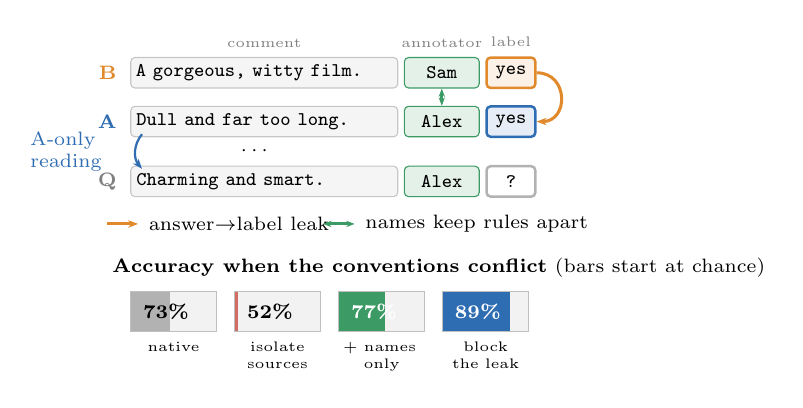
\begin{tikzpicture}[
  chip/.style={rounded corners=1.5pt, inner sep=2pt, minimum height=11pt, font=\scriptsize\ttfamily, anchor=west, line width=.4pt},
  cmt/.style={chip, draw=gray!45, fill=gray!8, text width=3.25cm, align=left},
  nm/.style={chip, draw=nameC, fill=nameC!14, minimum width=.95cm, align=center},
  ans/.style={chip, line width=.9pt, minimum width=.62cm, align=center},
  tag/.style={font=\scriptsize\bfseries, anchor=east},
  flow/.style={-{Stealth[length=3.6pt]}, rounded corners=3pt},
  note/.style={font=\scriptsize, align=left, inner sep=1pt}]
% rows
\foreach \y/\who/\c/\n/\a/\col in {0/B/A gorgeous{,} witty film./Sam/yes/srcB, -0.62/A/Dull and far too long./Alex/yes/srcA}{
  \node[cmt] (c\who) at (0,\y) {\c};
  \node[nm, right=2pt of c\who] (n\who) {\n};
  \node[ans, draw=\col, fill=\col!12, right=2pt of n\who] (a\who) {\a};
  \node[tag, text=\col] at ($(c\who.west)+(-.05,0)$) {\who};
}
\node[font=\scriptsize] at (1.6,-1.0) {$\cdots$};
\node[cmt] (cQ) at (0,-1.38) {Charming and smart.};
\node[nm, right=2pt of cQ] (nQ) {Alex};
\node[ans, draw=gray!60, fill=white, right=2pt of nQ] (aQ) {\textbf{?}};
\node[tag, text=gray] at ($(cQ.west)+(-.05,0)$) {Q};
% column headers
\node[font=\tiny, text=gray, above=0pt of cB] {comment};
\node[font=\tiny, text=gray, above=0pt of nB] {annotator};
\node[font=\tiny, text=gray, above=0pt of aB] {label};
% mechanism 1: B's answer leaks into A's label position
\draw[flow, srcB, line width=1.1pt] (aB.east) to[out=0, in=0, looseness=1.7] (aA.east);
% mechanism 2: names tell the sources apart
\draw[nameC, line width=1.1pt, {Stealth[length=3pt]}-{Stealth[length=3pt]}] (nB.south) -- (nA.north);
% legend
\begin{scope}[shift={(-.3,-1.92)}, font=\scriptsize]
\draw[flow, srcB, line width=1.1pt] (0,0) -- (.4,0) node[right, text=black] {answer$\to$label leak};
\draw[nameC, line width=1.1pt, {Stealth[length=3pt]}-{Stealth[length=3pt]}] (2.75,0) -- (3.15,0) node[right, text=black] {names keep rules apart};
\end{scope}
% reading
\draw[flow, srcA, line width=.8pt] ($(cA.west)+(.15,-.16)$) to[out=-130, in=130] ($(cQ.west)+(.15,.16)$);
\node[note, text=srcA, anchor=east] at (-.32,-1.0) {A-only\\reading};
% result strip
\begin{scope}[shift={(0,-2.78)}]
\node[font=\scriptsize, anchor=west] at (-.35,.3) {\textbf{Accuracy when the conventions conflict} (bars start at chance)};
\foreach \x/\v/\lab/\col/\tc in {0/73/native/gray!60/black, 1.32/52/isolate sources/blk!80/black, 2.64/77/+ names only/nameC/white, 3.96/89/block the leak/srcA/white}{
  \fill[gray!10] (\x,0) rectangle ++(1.1,-.5);
  \fill[\col] (\x,-.5) rectangle ++({1.1*(\v-50)/50},.5);
  \draw[gray!50, line width=.3pt] (\x+.0,-.5) rectangle ++(1.1,.5);
  \node[font=\scriptsize\bfseries, text=\tc, anchor=west] at (\x+.04,-.25) {\v\%};
  \node[font=\tiny, anchor=north, text width=1.2cm, align=center] at (\x+.55,-.52) {\lab};
}
\end{scope}
\end{tikzpicture}}
\caption{Two annotators label reviews with the same words but opposite conventions: Sam uses \lw{yes} for positive reviews, Alex for negative ones, and the query asks for Alex's label.
While the prompt is processed, Alex's label position reads Sam's earlier answer and absorbs Sam's rule, so restricting the query to Alex's demonstrations does not isolate Alex's rule (\S\ref{sec:observation}--\S\ref{sec:path}).
Attention between the annotators' names is what lets the model keep the two rules apart (\S\ref{sec:consequences}).
Bottom: SST-5 accuracy under conflicting conventions, averaged over our \nmodels{} models.}
\label{fig:overview}
\end{figure}

\section{Introduction}

In-context learning lets a language model infer a task from a handful of demonstrations \citep{brown2020language}.
In practice the demonstrations in a prompt often come from more than one source.
Annotators disagree in systematic ways on subjective tasks, and the variation they produce is a signal to be modelled rather than noise to be averaged away \citep{plank-2022-problem,davani-etal-2022-dealing,sachdeva-etal-2022-measuring}.
When the labelled examples of several annotators share one prompt, each annotator's examples encode a different rule over the same label words, and a model asked how a particular annotator would label a new input has to apply that annotator's rule.
Figure~\ref{fig:overview} shows a minimal case: two annotators judge the sentiment of movie reviews, one answers \lw{yes} for positive reviews and the other for negative ones, and the query asks for the second annotator's label.

Mechanistic studies of in-context learning describe how a demonstrated rule reaches the prediction.
Information about each input flows into the label position of its demonstration while the prompt is processed, and the query later retrieves the task from these label positions \citep{wang-etal-2023-label,cho2025revisitingincontextlearninginference}.
This account suggests a direct way to make a model use one source's rule, and one that context-isolation methods implement for other purposes \citep{ratner-etal-2023-parallel}: restrict the query to the demonstrations of the requested source, so that the label positions of other sources are never read.

The states at a label position, however, are themselves computed by attending to everything earlier in the prompt.
Demonstrations are contextualized by the demonstrations that precede them before their information is aggregated \citep{bakalova2025contextualizethenaggregatecircuitsincontextlearning}, and in a pooled prompt the preceding demonstrations include those of the other source.
If the label positions of one source take in the rule of another, a query that reads only the requested source still receives the other source's rule, now located at the requested source's positions.
Whether this happens matters for how in-context behaviour is attributed to demonstrations and for how sources should be kept apart.
It also raises a second question.
A model that answers correctly for each source must at some point associate each rule with its source, and the interactions between sources during prompt processing are a natural place for that to happen.
This paper asks how the computation that processes a multi-source prompt mixes the sources' rules, and how it separates them.

We study prompts in which two sources follow different conventions for the same task, change one source's rule while holding the other source's demonstrations and the query fixed, and intervene on attention in \nmodels{} frozen models from the Qwen3, Mistral, Llama and Gemma families with 2B to 70B parameters.
We separate two stages of the computation: the \emph{formation} of demonstration states while the prompt is processed, and their \emph{reading} by the query.
Our main experiments use reviews from SST-5 \citep{socher-etal-2013-recursive}, and controlled tasks with templated reviews let us vary the rules independently of the text.

Our findings fit together as follows.
When the two sources share label words, the other source's convention shifts the model's predictions for the requested source even when the query cannot attend to the other source, whichever pair of words they share, while with separate label words the shift vanishes (\S\ref{sec:observation}).
The shift travels mainly through one attention path in the first half of the network: the label positions of the requested source read the earlier \emph{answers} of the other source.
Replacing only the keys of these answer messages reproduces how separate label words change the requested source's label states, with a coefficient of one ($r=$ 0.80--0.95), blocking them in the ordinary forward pass removes 35--94\% of the cross-source effect, and the messages carry the other source's input--label association rather than only its label words (\S\ref{sec:path}).
Cross-source formation also does necessary work.
Removing all of it leaves each source's rule intact but makes the model unable to tell the rules apart: with conflicting conventions its predictions fall to chance, and with separate label words it answers in the other source's vocabulary about half of the time.
Attention to the other source's names, a few tokens per demonstration, restores most of the distinction, whereas the far more numerous comment tokens do not.
Blocking only the answer-to-label path keeps the rules apart and removes most of the leak, improving accuracy in every model, and public information about the sources helps only when it is available during formation (\S\ref{sec:consequences}).

Our contributions are as follows.
(1) We show that restricting the query to one source does not isolate that source's rule in pooled prompts with shared label words, and we identify the answer-to-label attention path that carries the other source's rule, with a prediction that needs no fitted parameters and with necessity and sufficiency tests in the native computation.
(2) We show that the same cross-source formation that mixes the rules is what allows the model to assign them to their sources, and that attention to the other source's names carries most of this function, so that isolating the sources completely leaves the rules learned but unusable.
(3) We show that blocking a single attention path during formation improves source-conditioned accuracy in all \nmodels{} models, and that shared information helps only through formation, which yields concrete guidance for interpreting and controlling multi-source prompts.

\section{Setup}
\label{sec:setup}

\paragraph{Sources and rules.}
Each prompt contains demonstrations from two sources, A and B, eight from each in random interleaved order, followed by queries.
A demonstration consists of a comment, the name of the annotator, and a label word (Figure~\ref{fig:overview}). A query has the same fields and ends after \texttt{Label:}, so the model's next token is its answer.
Each source follows a \emph{convention}, which states which of its two label words it uses for positive inputs, and the model has to infer each convention from the demonstrations.
In the \emph{same-convention} world both sources map positive inputs to the same word, and in the \emph{opposite-convention} world they map them to different words.
With \emph{shared} label words both sources answer with \lw{no}/\lw{yes}, and with \emph{separate} label words B answers with \lw{pass}/\lw{flag} while A keeps \lw{no}/\lw{yes}.
In every comparison A's comments, labels and positions and the queries stay fixed, and only B's demonstrations change.

\paragraph{Data.}
The main experiments use the most extreme classes of SST-5 \citep{socher-etal-2013-recursive} as positive and negative movie reviews.
Demonstrations come from the training split, and queries from the validation split during development and from the test split for all reported results.
Controlled experiments use templated restaurant reviews, which let us keep B's label sequence and comment set fixed while reassigning comments between classes.
A further variant has comments with independent food and service sentiment and sources that differ in the aspect they judge, and we use comments from the Measuring Hate Speech corpus \citep{sachdeva-etal-2022-measuring} for replications (Appendix~\ref{app:materials}).

\paragraph{Models.}
We use Qwen3-8B, 14B and 32B \citep{yang2025qwen3}, Mistral-7B-v0.3 \citep{jiang2023mistral}, Llama-3.1-8B and 70B \citep{grattafiori2024llama} and Gemma-2-2B and 9B \citep{gemma2024gemma2}, without chat templates and with frozen weights, FP32 computation and exact attention (Appendix~\ref{app:models}).

\paragraph{Formation and reading.}
The \emph{label position} of a demonstration is the first token of its label word, and its \emph{answer tokens} are the label word and the line breaks after it.
Under causal attention, the states at each demonstration token are computed from all earlier tokens.
We call this computation the \emph{formation} of demonstration states, and the query's attention to them \emph{reading}.
We intervene on either stage by removing attention edges: at every layer and head, the attention score from a receiving token to a set of earlier tokens is set to $-\infty$ before the softmax, the remaining attention is renormalized, and all later states are recomputed.
\emph{A-only reading} removes the edges from every query token to all of B's tokens, so that the query reads only the shared header and A's demonstrations.
Interventions on formation remove edges between the two sources' demonstrations and are described where they are used.

\paragraph{Measuring a cross-source effect.}
Let $z(q)$ be the logit of A's second label word minus that of its first at query $q$, and $g_A(q)\in\{-1,+1\}$ the sign of A's correct answer.
The effect of B's convention on A's predictions is
\begin{equation}
\Delta = \tfrac{1}{2}\,\mathbb{E}_q\!\left[g_A(q)\big(z_{\text{same}}(q)-z_{\text{opp}}(q)\big)\right],
\label{eq:delta}
\end{equation}
where the subscripts give B's convention and A's demonstrations are identical in both worlds.
$\Delta$ is measured in nats, and a positive value means that A's predictions are pulled toward B's convention: they are more correct when B agrees with A and less correct when it does not.
Accuracy counts a query as correct when the highest-scoring token in the full vocabulary is the requested source's correct label word, averaged over both requested sources, both convention worlds and all queries.

\paragraph{Evaluation.}
The unit of analysis is a prompt with its eight queries.
For each experiment we fixed the conditions and analyses on 16 development prompts and then ran them once on 32 new prompts with new material, from which all reported numbers come.
Intervals are 95\% percentile intervals from 10{,}000 bootstrap resamples of prompts.
Analyses added after the confirmation runs are marked in the appendix, and code for all experiments is provided in the supplementary material.

\section{Restricting the query does not isolate a source}
\label{sec:observation}

\begin{figure}[t]
\centering
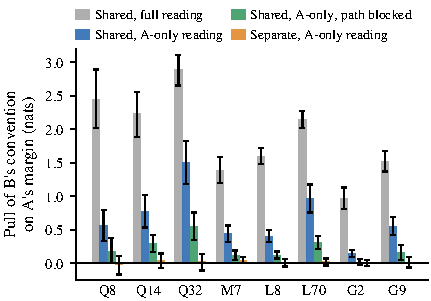
\includegraphics[width=\columnwidth]{figures/fig_leak}
\caption{Pull of B's convention on predictions for A ($\Delta$, Eq.~\ref{eq:delta}) on SST-5 reviews.
When the query can read only A's demonstrations, B's convention still shifts A's predictions if the two sources share label words (blue), and blocking the answer-to-label path during formation removes most of the remaining effect (green).
With separate label words the effect vanishes (orange).
Q, M, L, G: Qwen3, Mistral, Llama-3.1, Gemma-2 with size in billions. Error bars: 95\% intervals over 32 prompts.}
\label{fig:leak}
\end{figure}

Figure~\ref{fig:leak} shows how B's convention affects predictions for A.
When the query reads both sources, the pull is large, between 1.0 and 2.9 nats, because the query sees B's demonstrations directly.
A-only reading removes this direct access, yet B's convention still shifts A's predictions by 0.14 to 1.50 nats in all eight models.
In five of them the shift changes answers: A's answers are 2.3 to 7.4 points less accurate when B's convention conflicts with A's than when it agrees, although A's demonstrations and the queries are the same in both prompts. In Qwen3-14B and the two Gemma models the shift in A's margin does not reach the accuracy.
Changing B's demonstrations without changing B's association, by exchanging comments within the same class, produces no such shift (between $-0.21$ and $0.10$ nats, with intervals that include zero in every model), so the effect reflects B's rule and not a change in B's text.
In the controlled reviews the same restriction leaves an effect of 0.74 to 1.71 nats (Table~\ref{tab:operation}), and in Measuring Hate Speech comments B's rule changes 17.6\% of Qwen3-8B's answers for A (Appendix~\ref{app:observation}).

The effect depends on the label words.
When B answers with \lw{pass}/\lw{flag}, the pull of B's convention on A's predictions under A-only reading vanishes ($-0.03$ to $0.04$ nats), although the query still reads the same A demonstrations and B's demonstrations still precede them.
The change in A's margin per query, regardless of direction, then falls to 0.11--0.41 nats, the size produced by exchanging B's comments within class (0.09--0.32), whereas with shared words it is 0.17--1.58 nats (Appendix~\ref{app:observation}).
What matters is whether the words are shared, not which words: when both sources answer with \lw{pass}/\lw{flag} the pull is 0.39--1.01 nats, and when A answers with \lw{pass}/\lw{flag} and B with \lw{no}/\lw{yes} it is 0.04--0.10 (Appendix~\ref{app:edges}).
Within each family the pull is larger in the larger model, also when the 8B models are run on exactly the prompts used for Qwen3-32B and Llama-3.1-70B (from 0.65 to 1.50 and from 0.57 to 0.96 nats; Appendix~\ref{app:observation}).

Since the query in this setting reads only A's tokens, B's rule must reach the prediction through the states at A's positions, which were formed while B's demonstrations were in context.
The next section identifies the attention path through which it gets there.

\section{The answer-to-label path}
\label{sec:path}

A label position is the natural place to look.
It holds the task information that the query retrieves \citep{wang-etal-2023-label,cho2025revisitingincontextlearninginference}, and when it is computed it can attend to the answers of all earlier demonstrations, including B's.
We call the attention from A's label positions to B's earlier answer tokens the \emph{answer-to-label path}.
We test whether this path carries B's rule in three ways: whether it predicts the effect of B's label words, whether the native computation depends on it, and what it carries.

\begin{figure*}[t]
\centering
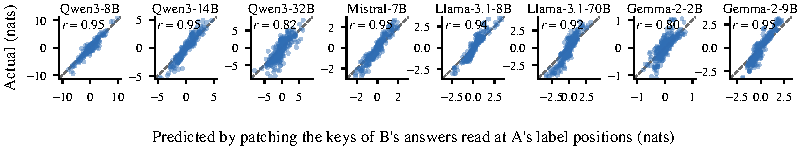
\includegraphics[width=\textwidth]{figures/fig_reconstruction}
\caption{Patching the answer-to-label path predicts how B's label words change A's label states (SST-5, A-only reading).
Each point is one query (32 prompts $\times$ 8 queries); the effect is the difference between B's two conventions of the change caused by replacing A's label states with those formed when B uses separate label words.
The prediction replaces only the keys that A's label positions read at B's answer tokens.
The dashed line is the identity: no parameter is fitted.}
\label{fig:reconstruction}
\end{figure*}

\subsection{The path predicts the effect of the label words}

If B's convention reaches A's label states through what they read at B's answers, then the change that separate label words make to A's label states should be reproduced by changing only these messages.
Both sides of this comparison are interventions on A's label states.
The \emph{effect} transplants the states of A's label tokens from a run in which B uses separate label words into the shared-word prompt.
The \emph{prediction} keeps the shared-word prompt and replaces only the keys (or keys and values) that A's label tokens read at B's answer tokens, at every layer, with those of the separate-word run, and all later states are recomputed.
Both are read out at the query's prediction for A as the difference between B's two conventions, which removes any shift that does not depend on B's rule, and the prediction has a coefficient of one and no fitted parameter \citep[cf.][]{zhang2024towards}.

Under A-only reading, the setting of \S\ref{sec:observation}, the prediction from keys alone matches the effect closely (Figure~\ref{fig:reconstruction}).
Correlations are 0.92 to 0.95 in six models and 0.82 and 0.80 in Qwen3-32B and Gemma-2-2B, with points along the identity line.
When the query reads both sources, patching keys and values predicts the effect with $r=0.92$--$0.99$ in seven models and $0.72$ in Llama-3.1-70B, whose A states then compete with B's directly readable states (Appendix~\ref{app:reconstruction}).
Patching keys alone recovers most of the effect and patching values alone recovers less, so B's label words change where A's label positions attend among B's answers as well as what they receive.
On Measuring Hate Speech comments the prediction reaches $r>0.97$ for Qwen3-8B and Mistral-7B.

\begin{table}[t]
\centering\small
\setlength{\tabcolsep}{4pt}
\adjustbox{max width=\columnwidth}{\begin{tabular}{@{}lccc@{}}
\toprule
 & \makecell{Effect with\\A-only reading} & \makecell{Reduction when\\path is removed} & \makecell{Effect with\\only the path} \\
\midrule
Qwen3-8B      & 1.14 & 0.55 & 0.73 \\
Qwen3-14B     & 1.63 & 0.56 & 0.56 \\
Qwen3-32B     & 1.71 & 0.89 & 0.39 \\
Mistral-7B    & 0.74 & 0.52 & 0.32 \\
Llama-3.1-8B  & 0.94 & 0.55 & 0.48 \\
Llama-3.1-70B & 0.98 & 0.59 & 0.40 \\
Gemma-2-2B    & 0.20 & 0.19 & 0.12 \\
Gemma-2-9B    & 0.79 & 0.50 & 0.30 \\
\bottomrule
\end{tabular}}
\caption{The answer-to-label path in the native computation (controlled reviews, shared label words, A-only reading).
Effect: $\Delta$ (Eq.~\ref{eq:delta}, nats).
Reduction: decrease of this effect when A's label positions cannot attend to B's answers during formation.
Only the path: effect when A's demonstrations can attend to B's only through this path (zero without it).
All 95\% intervals exclude zero (Appendix~\ref{app:operation}).}
\label{tab:operation}
\end{table}

\subsection{The native computation depends on the path}
\label{sec:native}

A successful prediction shows that the path can carry the effect, not that the model's own computation uses it.
We therefore intervene on the ordinary forward pass without any donor states (Table~\ref{tab:operation}).
Removing the answer-to-label path while the prompt is processed reduces the effect of B's rule under A-only reading by 0.19 to 0.89 nats, between 35\% and 94\% of the total, in all eight models, and on SST-5 blocking it in both directions removes 62--93\% (Figure~\ref{fig:leak}, green).
Conversely, when we block all attention from A's demonstrations to B's and then reopen only this path, B's rule again affects A's predictions, by 0.12 to 0.73 nats, a quarter to two thirds of the full effect.
Blocking the path in one quarter of the layers at a time shows where it acts: most of the reduction comes from the second quarter of the layers and none from the last, in each of the six models where we measured it (Appendix~\ref{app:edges}).
The path is thus both a substantial part of the native route and sufficient on its own to transmit B's rule.
The remainder of the effect travels through other cross-source edges, such as attention from A's comments to B's demonstrations.
The reduction is specific to B's answers: blocking A's label positions from A's \emph{own} earlier answers does not reduce the effect of B's rule in any model and increases it in seven of the eight, by 0.12 to 0.68 nats (Appendix~\ref{app:operation}).

When the query can also read B directly, A's evidence competes with B's own states, and the net contribution of the path differs in sign between models (Appendix~\ref{app:operation}).

\subsection{The path carries the association, not only the words}
\label{sec:assoc}

Separating the label words changes both which words B uses and how B's answers relate to its comments, so the reconstruction alone does not show which of the two the path carries.
To isolate the association, we keep B's label sequence, positions and comment set fixed and reverse its association by exchanging comments between B's positive and negative demonstrations.
As a control we exchange the same number of comments within each class, which moves text without changing the association.
We patch only the answer messages that A's label positions receive from each modified prompt into the original prompt.

Messages from the reversed association change A's predictions more than messages from the control, by 0.62 and 0.40 nats in Qwen3-8B and Mistral-7B on controlled reviews and by 0.03 to 0.49 nats in all eight models on SST-5 (Appendix~\ref{app:association}).
The answer messages transmit B's input--label association even though every label word stays in place.
The sign of this change differs between families (positive in the Qwen3, Mistral and Gemma models, negative in both Llama models): the path delivers B's association to A's label states, and how these states combine it with A's own demonstrations depends on the model.

\section{Cross-source formation also separates the rules}
\label{sec:consequences}

If cross-source formation only leaked rules between sources, removing it should help.
We compare three ways of separating the sources on SST-5 (Table~\ref{tab:policies}).
\emph{Selective blocking} removes the answer-to-label path in both directions while the prompt is processed and keeps all other attention.
\emph{Complete isolation} removes all attention between the two sources' demonstrations while the prompt is processed, so that each source is encoded as if it were alone.
\emph{A-only reading} restricts the query, as in \S\ref{sec:observation}, and is applied for each requested source in turn, which requires knowing at query time which tokens belong to which source.

\begin{table}[t]
\centering\small
\setlength{\tabcolsep}{2.6pt}
\adjustbox{max width=\columnwidth}{\begin{tabular}{@{}lccccc@{}}
\toprule
 & Native & \makecell{Selective\\blocking} & \makecell{Complete\\isolation} & \makecell{A-only\\reading} & \makecell{Instruc-\\tion} \\
\midrule
Qwen3-8B      & 84.9 & \textbf{+7.3}  & $-$9.9  & \ns{$-$0.4} & +2.3 \\
Qwen3-14B     & 89.9 & \textbf{+7.4}  & $-$14.9 & +3.8 & +1.7 \\
Qwen3-32B     & 88.0 & \textbf{+7.7}  & $-$12.7 & +5.9 & +5.7 \\
Mistral-7B    & 88.8 & +5.4  & $-$15.2 & \textbf{+6.0} & \ns{+1.0} \\
Llama-3.1-8B  & 81.3 & +9.5  & $-$6.1  & \textbf{+16.7} & +1.2 \\
Llama-3.1-70B & 88.5 & \textbf{+10.4} & $-$12.6 & +7.3 & +6.2 \\
Gemma-2-2B    & 85.3 & +2.5  & $-$10.6 & \textbf{+10.2} & \ns{$-$0.6} \\
Gemma-2-9B    & 89.9 & +7.7  & $-$14.8 & \textbf{+8.7} & \ns{+1.0} \\
\bottomrule
\end{tabular}}
\caption{Accuracy (\%) on SST-5 with shared label words, averaged over both requested sources and both convention worlds, and change in points under three ways of separating the sources and under a one-sentence instruction to use only the requested annotator's examples.
Bold: largest gain per model.
Gray: 95\% interval includes zero; all other changes exclude zero (Appendix~\ref{app:policies}).}
\label{tab:policies}
\end{table}

\paragraph{Selective blocking improves accuracy.}
Blocking the answer-to-label path improves accuracy in every model, by 2.5 to 10.4 points, and in seven of the eight it does so for each of the two requested sources separately.
The gain comes from prompts in which the sources' conventions conflict, where accuracy rises by 5.9 to 20.9 points (for example from 77.3\% to 98.2\% in Llama-3.1-70B), while prompts with agreeing conventions, already near ceiling, are unaffected.
On the controlled reviews with two aspects, where the sources can also differ in which aspect they judge, selective blocking improves accuracy by 2.8 to 7.4 points in the four models tested (Appendix~\ref{app:policies}).
A-only reading helps some models more and others less: it adds 16.7 points for Llama-3.1-8B and nothing for Qwen3-8B.
The two interventions act on different stages, and selective blocking needs no restriction of the query.
An explicit instruction to use only the requested annotator's examples helps less than selective blocking in seven of the eight models.
A prompt that contains only the requested source's demonstrations reaches 94.8--99.3\%, and selective blocking closes between a quarter (Gemma-2-2B) and nearly all (96\%, Llama-3.1-70B) of the gap between the pooled prompt and this single-source prompt.

\begin{figure*}[t]
\centering
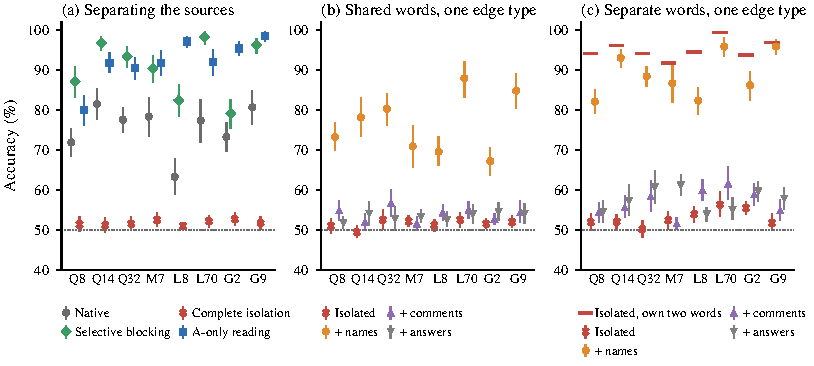
\includegraphics[width=\textwidth]{figures/fig_separation}
\caption{What separates the two sources' rules (SST-5, conflicting conventions unless noted).
(a) Complete isolation leaves the model at chance, while selective blocking raises accuracy above the native level.
(b, c) Starting from complete isolation, letting each source see only the other source's \emph{names} restores most of the separation, with shared words (b) and with separate words (c, full-vocabulary accuracy over both convention worlds), whereas the far more numerous comment tokens or the answers do not.
The dash in (c) marks accuracy under complete isolation when the answer is restricted to the requested source's own two words.
Model labels as in Figure~\ref{fig:leak}; error bars: 95\% bootstrap intervals.}
\label{fig:separation}
\end{figure*}

\paragraph{Complete isolation makes the rules indistinguishable.}
Removing all cross-source attention during formation lowers accuracy below the native level in every model, to about 75\%.
The breakdown by world explains this number (Figure~\ref{fig:separation}a).
With agreeing conventions accuracy stays at 94--100\%, and with conflicting conventions it falls to 51--53\%, which is chance.
The rules themselves are intact: under complete isolation combined with A-only reading accuracy is 93--99\%.
What complete isolation removes is the model's ability to use the source named in the query to choose between two rules that it has learned.
Selective blocking keeps this ability, reaching 79--98\% with conflicting conventions.



\paragraph{Separate label words show what is lost.}
With separate label words, complete isolation still leaves 94--99\% of answers correct when the decision is restricted to the requested source's two words, as accurate as the native model (Figure~\ref{fig:separation}c).
The model's actual answers are correct only 52--56\% of the time, because in 42--47\% of queries it answers with the other source's words.
Without cross-source formation the model knows each rule but not which label space belongs to the source it is asked about.
Accuracy restricted to a source's own words, the usual way of scoring classification by in-context learning, would not reveal this failure.

\paragraph{The other source's names do the separating.}
Complete isolation removes three kinds of cross-source attention at once: to the other source's comments, to its names and to its answers.
To find out which of them the model needs, we start from complete isolation and let every token of a source attend again to one kind of the other source's tokens, using new prompts (Figure~\ref{fig:separation}b, c; Appendix~\ref{app:edges}).
Reopening the names, about five tokens per demonstration, raises accuracy under conflicting conventions from 49--53\% to 67--88\%, above the native prompt in five of the eight models, and with separate words it raises full-vocabulary accuracy from 50--56\% to 82--96\%.
Reopening the comments, which contain several times more tokens, or the answers leaves accuracy at 52--62\%, so what complete isolation removes is not context in general.
The model needs each source's demonstrations to be formed in view of the other source's identity, and the name in the query then selects between the two rules.

\begin{figure}[t]
\centering
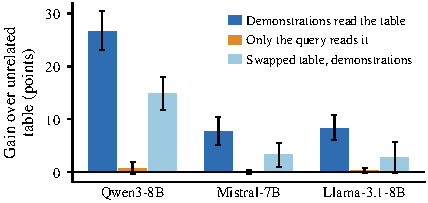
\includegraphics[width=\columnwidth]{figures/fig_schema}
\caption{A public table listing each source's label words (e.g., \texttt{Alex: no, yes; Sam: pass, flag}) helps when the demonstrations can read it during formation and not when only the query can read it.
Private cross-source attention is blocked throughout. Gains are relative to a table with unrelated names, and error bars are 95\% bootstrap intervals.}
\label{fig:schema}
\end{figure}

\paragraph{Shared information helps through formation.}
If cross-source formation supplies the link between sources and their rules, that link should be replaceable by explicit shared information, and it should matter when that information is available.
We keep private cross-source attention blocked and add, before all demonstrations, a public table that lists each source's two label words without any demonstrations, then control separately whether demonstrations can read the table during formation and whether the query can read it.
When only the demonstrations can read the table, full-vocabulary accuracy rises by 26.7, 7.7 and 8.3 points over a table with unrelated names in Qwen3-8B, Mistral-7B and Llama-3.1-8B (Figure~\ref{fig:schema}).
When only the query can read it, the gain is at most 0.8 points, with intervals that include zero.
The table helps by shaping how each source's demonstrations are encoded, not by being looked up at query time.
A table with the two sources' word sets swapped also helps in Qwen3-8B and Mistral-7B (by 14.9 and 3.3 points over the unrelated table), though less than the correct table, so the demonstrations do not simply follow the table's assignment (Appendix~\ref{app:shared}).
The encodings must also be common: states of the two sources taken from two separate encodings of the same facts are used less well than states from one encoding (Appendix~\ref{app:shared}).

\section{Discussion}
\label{sec:discussion}

\paragraph{Why shared label words matter.}
Three observations identify the label word as the link between the sources.
The cross-source effect appears whenever the sources share label words, whether both use \lw{no}/\lw{yes} or both use \lw{pass}/\lw{flag}, and vanishes when their words differ in either assignment.
Patching keys alone reproduces most of the effect of separating the words.
And A's label positions place more attention on B's answers when the words are shared (0.3 to 2.3 percentage points of attention mass, Appendix~\ref{app:edges}).
A label position thus treats earlier answers that carry its own label words as further instances of its label and takes in the comments that go with them, whichever source gave them, which extends the role of label words as anchors \citep{wang-etal-2023-label,zheng-etal-2026-label} across sources.

\paragraph{Two kinds of cross-source interaction.}
Formation passes two different things between the sources.
Through the answers it passes the other source's input--label association, which mixes the rules, and through the names it passes what lets the query tell the rules apart.
The two travel on different tokens and can be separated by intervention, as selective blocking does.
Methods that encode sources independently, such as parallel context windows, remove both, and methods that only restrict what the query reads remove neither.
Both of our interventions use the token ownership that structured prompts provide.

\section{Related Work}
\label{sec:related}

\paragraph{Mechanisms of in-context learning.}
Information about demonstrations is aggregated at label positions and read out by the query \citep{wang-etal-2023-label}, through circuits that encode inputs, merge them into label states and retrieve them \citep{cho2025revisitingincontextlearninginference,cho2026mechanismtaskorientedinformationremoval}.
Demonstrations are contextualized by earlier ones before aggregation \citep{bakalova2025contextualizethenaggregatecircuitsincontextlearning}, and task information is carried by function and task vectors \citep{todd2024function,hendel-etal-2023-context,wang2026fewshotexamplesaddup}, label words \citep{zheng-etal-2026-label} and representations that appear just in time \citep{li2025justintimedistributedtaskrepresentations}.
Input--label mappings have been traced to specific heads \citep{sun-etal-2025-interpret,yu-ananiadou-2024-large,olsson2022context,crosbie-shutova-2025-induction}.
These studies analyse one task per prompt. We study prompts in which label positions also hold other sources' rules.

\paragraph{Labels and rules in context.}
Models use the input--label mapping of demonstrations to different degrees \citep{min-etal-2022-rethinking,kossen2024incontext}, larger models can follow flipped labels \citep{wei2023larger}, label words carry prior biases \citep{zhao2021calibrate}, and several tasks can be run in superposition from one prompt \citep{xiong2024everything,li-etal-2024-language,yang2026localizingtaskrecognitiontask}.
Conflicting demonstrations \citep{jiao2026understandingdynamicsdemonstrationconflict} and conflicts with prior knowledge \citep{li2026contextmisleadsincontextlearning} have been studied as errors, whereas our two rules are both legitimate.
Models also struggle to use representations learned in context \citep{lepori-etal-2026-language}, in line with rules that complete isolation leaves learned but unusable.

\paragraph{Binding, annotators and isolation.}
Models bind entities to attributes through binding IDs \citep{feng2024languagemodelsbindentities,dai-etal-2024-representational}, retrieve them through several interacting mechanisms \citep{gurarieh2026mixingmechanismslanguagemodels,thavarasa2026testroutelanguagemodels} and err when entities are contextualized late \citep{lepori-etal-2025-racing}. Linking a rule to its source is a binding problem of this kind, and in our prompts it is solved during formation through the sources' names.
Annotator disagreement carries information worth modelling \citep{plank-2022-problem,davani-etal-2022-dealing,santurkar2023whose}, and pooling annotators' examples in one prompt is a natural way to do so with in-context learning.
Parallel context windows and structured prompting encode groups of demonstrations separately \citep{ratner-etal-2023-parallel,hao2022structured}, and KV-cache reuse recomputes part of the attention between independently encoded documents \citep{yao2025cacheblendfastlargelanguage}. Our results show that such isolation keeps rules from mixing but also removes what assigns them to their sources.
Our interventions build on attention knockout and activation patching \citep{geva-etal-2023-dissecting,zhang2024towards}.

\section{Conclusion}

In a prompt that pools the demonstrations of several sources, the evidence at a source's positions is formed in the presence of the other sources, so where the query reads does not determine whose rule it uses.
When sources share label words, the other source's association reaches the requested source's label states through attention to its earlier answers, and a coefficient-one patch of these messages predicts the effect of the shared words.
The same interaction during prompt processing also lets the model link each rule to its source, mainly through attention to the other source's names, which is why complete isolation leaves the rules learned but unusable and why shared information helps only when it is present during formation.
Separating sources in a pooled prompt therefore means deciding which cross-source interactions to keep, and removing only the answer-to-label path improved accuracy in every model.

\section*{Limitations}

The sources in our experiments follow conventions and aspect criteria that we assign over real and templated comments, which lets us change one rule while holding everything else fixed. The rules of real annotators can differ in several respects at once.
All tasks are binary, with two sources and eight demonstrations each, and prompts with more sources or labels may show stronger or weaker interaction.
Our interventions act on attention edges across all heads, so they identify paths and the layers that carry them rather than individual heads.
The eight models differ in training recipe as well as size, so comparisons across sizes describe these checkpoints.

\section*{Ethical Considerations}

We analyse publicly released models and datasets under their licenses (Appendix~\ref{app:models}).
The Measuring Hate Speech corpus contains offensive language. We use its comments only as model inputs, without annotator information, and show none of them in the paper.
The source-specific rules are synthetic and are not attributed to the original annotators.
Our interventions require white-box access to a model and are tools for analysis. Insight into how sources mix could also be used to make a model follow one source's rule more closely, which is the intended use in settings such as modelling individual annotators.

\bibliography{references}

\appendix
\setcounter{dbltopnumber}{3}
\setcounter{topnumber}{3}
\renewcommand{\dbltopfraction}{0.95}
\renewcommand{\topfraction}{0.95}
\renewcommand{\textfraction}{0.05}
\renewcommand{\dblfloatpagefraction}{0.85}
\renewcommand{\floatpagefraction}{0.85}
% Appendix of main.tex. Tables in tables/app_*.tex are written by ../scripts/paper_figures_v2.py.

\section{Models and computation}
\label{app:models}

Table~\ref{tab:models} lists the checkpoints.
The Qwen3 models are the released post-trained hybrid checkpoints and the Mistral and Llama models are base models. All are used as plain continuation models, without chat templates or generated reasoning.
All computations use FP32 weights and activations with TF32 disabled, the eager (exact) attention implementation of Transformers, no quantization, and no gradient updates.
Qwen3-32B is split over two GPUs and Llama-3.1-70B over four GPUs of one node by contiguous layers.
Every intervention applies to all layers and all heads, and no layer or head is selected.

\begin{table}[!ht]
\centering\small
\setlength{\tabcolsep}{3pt}
\adjustbox{max width=\columnwidth}{\begin{tabular}{@{}ll@{}}
\toprule
Checkpoint & Revision \\
\midrule
Qwen/Qwen3-8B & \texttt{b968826d} \\
Qwen/Qwen3-14B & \texttt{40c06982} \\
Qwen/Qwen3-32B & \texttt{9216db57} \\
mistralai/Mistral-7B-v0.3 & \texttt{caa1feb0} \\
NousResearch/Meta-Llama-3.1-8B & \texttt{1f47e50c} \\
meta-llama/Llama-3.1-70B & \texttt{349b2ddb}$^\dagger$ \\
\bottomrule
\end{tabular}}
\caption{Model checkpoints (Hugging Face revisions, first eight characters).
$^\dagger$Loaded from the public mirror \texttt{NousResearch/Meta-Llama-3.1-70B}, whose 30 weight shards are byte-identical to this official revision.}
\label{tab:models}
\end{table}

Before scoring, we check for each model that every label word, with its leading space, is a single token; that scoring a query from the cached prompt agrees with scoring the full token sequence (maximum difference below $10^{-4}$ nats); that patching a run with its own states changes nothing; and that every attention mask is applied at every layer.
The experiments used about 80 GPU-hours on A100 and RTX PRO 6000 GPUs, most of them for the 32B and 70B models.

\section{Materials and prompt format}
\label{app:materials}

\paragraph{Prompt format.}
Every prompt starts with the header \texttt{Below are comments and the labels that individual annotators gave them.} followed by a blank line.
Each demonstration has three lines, \texttt{Comment:}, \texttt{Annotator:} and \texttt{Label:}, followed by a blank line, and each query ends after \texttt{Label:}.
The header, each demonstration up to the colon after \texttt{Label}, the label word and the separator are tokenized separately and concatenated, so that token boundaries are identical across all conditions that are compared.
The \emph{label position} of a demonstration is the first token of its label word, and its \emph{answer tokens} are the label word and the following separator tokens.
A source owns every token of its demonstrations, and the header belongs to neither source.
Each prompt has eight demonstrations per source in random order and eight queries, four positive and four negative.
Source names, the order of demonstrations and the direction of A's convention vary across prompts and are balanced.
Queries are scored in a batch from a copy of the processed prompt, with left padding and explicit position indices.

\paragraph{SST-5.}
We use the original classes 0 (very negative) and 4 (very positive) of SST-5 \citep{socher-etal-2013-recursive}, remove duplicate texts within each split, and keep reviews of 5 to 64 tokens.
Demonstrations for development and confirmation prompts come from the two halves of the training split defined by the parity of a hash of the text.
Queries come from the validation split for development and from the test split for confirmation, excluding any text that also appears in the training or validation split.
In the main experiments both sources judge sentiment and differ only in convention.

\paragraph{Controlled reviews.}
Single-aspect reviews are generated from templates (\textit{The pizza was outstanding.}).
They allow B's rule to be reversed without changing B's label sequence or comment set: for B's eight demonstrations we sample two quartets matched in length, each with two positive and two negative comments, and exchange the comments across classes (reversing the association) or within classes (the control).
Two-aspect reviews mention food and then service with independently chosen sentiment (\textit{The pasta was delicious, but the waiter was rude.}). A always judges food, and B judges food or service under the same or the opposite convention, giving four worlds.

\paragraph{Measuring Hate Speech.}
We group the corpus \citep{sachdeva-etal-2022-measuring} by comment, average the annotations, keep comments of at most 50 words with a mean hate-speech score of at least 1, and separate comments targeting race (race score at least 0.75, gender at most 0.1) from comments targeting gender (the reverse).
The two sources map the two target categories to \lw{safe}/\lw{toxic} with opposite conventions.
These rules are constructed and are not the rules of the original annotators.

\section{Interventions}
\label{app:interventions}

\paragraph{Edge removal.}
To remove the attention from a set of receiving tokens to a set of sending tokens, we set the corresponding pre-softmax attention scores to $-\infty$ at every layer and head.
Each token always keeps its attention to itself, and the remaining attention is renormalized.
\emph{Removing the answer-to-label path} blocks the attention from A's label positions to all earlier answer tokens of B.
The own-answer control blocks the attention from A's label positions to A's earlier answer tokens.
\emph{Restoring only the path} starts from a prompt in which no token of A attends to any token of B, and reopens the attention from A's label positions to B's earlier answer tokens.
\emph{Selective blocking} applies the answer-to-label removal in both directions (B's answers to A's label positions and A's answers to B's label positions) and \emph{complete isolation} removes all attention between the tokens of the two sources; in both cases the header remains visible to everyone.
\emph{Restricted reading} removes the attention from every query token to all tokens of the unrequested source.

\paragraph{Patching the answer-to-label path.}
For the predictions in \S\ref{sec:path}, a donor prompt differs from the recipient in B's label words (or, in \S\ref{sec:assoc}, in B's comment assignment).
At each layer, A's label positions in the recipient compute their attention with the recipient's queries and the full causal mask, but with keys, values or both at B's answer tokens taken from the donor's cache at that layer, including its positional encoding.
Only the outputs of these receiving positions change, and all later layers and positions are recomputed.
The effect to be predicted transplants the complete cached states of A's label positions from the donor into the processed recipient prompt and keeps all other positions.
Both are evaluated with the query reading both sources and are compared through the difference between B's two conventions, with a coefficient of one.

\section{Statistics}
\label{app:stats}

For each prompt we average over its eight queries, and all intervals resample prompts (10{,}000 percentile bootstrap draws), keeping all queries, worlds, requested sources and conditions of a prompt together.
Differences between conditions are computed within each prompt before resampling.
Correlations for the reconstruction are computed over all query-level points and resampled by prompt.
For each experiment, conditions and analyses were fixed on 16 development prompts and then run once on 32 new prompts with new material and new random seeds.
All numbers in the paper come from these confirmation prompts, and every condition that was run is reported here or in the main text.

\section{Additional results for Section~\ref{sec:observation}}
\label{app:observation}

Table~\ref{tab:app-leak} gives the values of Figure~\ref{fig:leak} with intervals, together with the control that exchanges B's comments within each class.
Table~\ref{tab:app-leak-matched} repeats the measurement for Qwen3-8B and Llama-3.1-8B on exactly the prompts used for Qwen3-32B and Llama-3.1-70B.
The accuracy differences in \S\ref{sec:observation} compare, for requests to A under A-only reading, prompts in which B's convention conflicts with A's and prompts in which it agrees. We computed this breakdown from the confirmation runs after they were completed.
The differences are 7.4 (3.5--11.7), 1.2 ($-3.1$--5.5), 7.4 (2.7--12.9), 7.4 (2.3--13.3), 2.3 (0.4--5.1) and 5.9 (2.0--10.5) points for Qwen3-8B, 14B, 32B, Mistral-7B, Llama-3.1-8B and 70B with shared words, and between $-1.2$ and 1.6 points with separate words.
When the query reads both sources, the differences with shared words are 10.5 to 30.9 points.
On Measuring Hate Speech comments with \lw{safe}/\lw{toxic} as shared label words and A-only reading, reversing B's convention changes 17.6\% (12.1--23.8) of Qwen3-8B's answers for A, with a mean absolute effect on A's margin of 0.73 nats.

\begin{table*}[t]
\centering\small
\adjustbox{max width=\textwidth}{\begin{tabular}{@{}lccccc@{}}
\toprule
 & \multicolumn{3}{c}{Shared label words} & Separate words & Control \\
\cmidrule(lr){2-4}\cmidrule(lr){5-5}\cmidrule(l){6-6}
 & Full reading & A-only reading & A-only, path blocked & A-only reading & within-class exchange \\
\midrule
\rows{tables/app_leak.tex}
\bottomrule
\end{tabular}}
\caption{Pull of B's convention on A's predictions ($\Delta$ in nats, SST-5) with 95\% intervals.
Control: B's comments are exchanged within each class, which leaves B's association unchanged (A-only reading, shared words).}
\label{tab:app-leak}
\end{table*}

\begin{table}[!ht]
\centering\small
\setlength{\tabcolsep}{2.5pt}
\adjustbox{max width=\columnwidth}{\begin{tabular}{@{}lccc@{}}
\toprule
 & Full & A-only & A-only, blocked \\
\midrule
\rows{tables/app_leak_matched.tex}
\bottomrule
\end{tabular}}
\caption{$\Delta$ (nats) on identical prompts within each family.}
\label{tab:app-leak-matched}
\end{table}

\section{Additional results for Section~\ref{sec:path}}

\subsection{Reconstruction}
\label{app:reconstruction}

Table~\ref{tab:app-recon} reports the reconstruction for each channel.
Patching keys alone predicts the effect nearly as well as patching keys and values, and patching values alone predicts it less well in every model.
The last column uses B states formed with separate label words as the reading background, which also gives high correlations.
Without taking the difference between B's two conventions, the KV correlations are 0.92, 0.95, 0.88, 0.86, 0.79 and 0.62 in the order of the table.
On Measuring Hate Speech comments the KV correlations of the convention difference are 0.985 for Qwen3-8B and 0.977 for Mistral-7B, with key-only correlations of 0.969 and 0.966.

\begin{table}[!ht]
\centering\small
\setlength{\tabcolsep}{2.4pt}
\adjustbox{max width=\columnwidth}{\begin{tabular}{@{}lccccccc@{}}
\toprule
 & K & V & KV & KV interval & RMSE & Zero & Sep. \\
\midrule
\rows{tables/app_reconstruction.tex}
\bottomrule
\end{tabular}}
\caption{Correlation between predicted and actual effects of B's label words on A's label states (difference between B's conventions, SST-5).
RMSE: error of the KV prediction (nats); Zero: error of predicting no effect; Sep.: KV correlation with B's separate-word states as reading background.}
\label{tab:app-recon}
\end{table}

\subsection{Native operation}
\label{app:operation}

Table~\ref{tab:app-op-gate} gives the values of Table~\ref{tab:operation} with intervals and adds the own-answer control.
Removing the attention from A's label positions to A's own earlier answers increases the effect of B's rule in every model, which shows that the reduction from removing the cross-source path is not a general consequence of disturbing the label positions.
Table~\ref{tab:app-op-full} gives the same quantities when the query reads both sources.
Removing the cross-source path still reduces B's effect in all models.
Restoring only the path, however, changes B's effect by different amounts and in different directions, because the query then also reads B's own states, and the path changes how A's states combine with them.

\begin{table*}[t]
\centering\small
\adjustbox{max width=\textwidth}{\begin{tabular}{@{}lcccc@{}}
\toprule
 & Effect & Reduction, cross-source path removed & Reduction, own-answer path removed & Effect with only the path \\
\midrule
\rows{tables/app_operation_gate.tex}
\bottomrule
\end{tabular}}
\caption{Native operation with A-only reading (controlled reviews, shared words; nats, 95\% intervals). A negative reduction is an increase.}
\label{tab:app-op-gate}
\end{table*}

\begin{table*}[t]
\centering\small
\adjustbox{max width=\textwidth}{\begin{tabular}{@{}lcccc@{}}
\toprule
 & Effect & Reduction, cross-source path removed & Reduction, own-answer path removed & Change when only the path is restored \\
\midrule
\rows{tables/app_operation_full.tex}
\bottomrule
\end{tabular}}
\caption{Native operation when the query reads both sources. Last column: effect with only the path minus effect with all attention from A to B blocked.}
\label{tab:app-op-full}
\end{table*}

\subsection{Association content}
\label{app:association}

Table~\ref{tab:app-assoc} reports how much more a reversal of B's association changes A's predictions than a matched exchange within classes.
In the full native prompt the excess is large, as expected, since the query also reads B's demonstrations.
Patching only A's label states, or only the answer messages they receive, transfers a smaller but reliable part of it in every model.
The signed effect of the answer messages differs in sign between families.
On controlled reviews with A-only reading, the excess for answer messages is 0.62 (0.45--0.81) nats for Qwen3-8B and 0.40 (0.31--0.50) for Mistral-7B, and values alone carry a substantial part of it.

\begin{table*}[t]
\centering\small
\adjustbox{max width=\textwidth}{\begin{tabular}{@{}lcccc@{}}
\toprule
 & Full prompt & A's label states patched & Answer messages patched & Answer messages, signed \\
\midrule
\rows{tables/app_association.tex}
\bottomrule
\end{tabular}}
\caption{Excess effect (nats) of reversing B's association over exchanging comments within classes, with B's label words and positions fixed (SST-5).
The first three columns compare absolute effects; the last column compares signed effects oriented by A's correct answer.}
\label{tab:app-assoc}
\end{table*}

\section{Additional results for Section~\ref{sec:consequences}}
\label{app:policies}

\paragraph{SST-5.}
Tables~\ref{tab:app-pol-acc}--\ref{tab:app-pol-other} report all six combinations of formation and reading for shared label words, the per-source and per-world changes under selective blocking, and the breakdown of complete isolation.
Table~\ref{tab:app-sep} reports separate label words.
For shared words, scoring the full vocabulary and scoring only the two label words give identical accuracies.

\begin{table*}[t]
\centering\small
\adjustbox{max width=\textwidth}{\begin{tabular}{@{}lcccccc@{}}
\toprule
 & & & & \multicolumn{3}{c}{A-only reading combined with} \\
\cmidrule(l){5-7}
 & Native & Selective blocking & Complete isolation & -- & Selective blocking & Complete isolation \\
\midrule
\rows{tables/app_policy_acc.tex}
\bottomrule
\end{tabular}}
\caption{Accuracy (\%) on SST-5 with shared label words for all combinations of formation and reading.}
\label{tab:app-pol-acc}
\end{table*}

\begin{table*}[t]
\centering\small
\adjustbox{max width=\textwidth}{\begin{tabular}{@{}lccccc@{}}
\toprule
 & Both sources & Source A & Source B & Opposite conventions & Same convention \\
\midrule
\rows{tables/app_policy_delta.tex}
\bottomrule
\end{tabular}}
\caption{Change in accuracy (points) from selective blocking, by requested source and by convention world.}
\label{tab:app-pol-delta}
\end{table*}

\begin{table*}[t]
\centering\small
\adjustbox{max width=\textwidth}{\begin{tabular}{@{}lccccc@{}}
\toprule
 & \multicolumn{2}{c}{Change vs.\ native (points)} & \multicolumn{2}{c}{Complete isolation (\%)} & Selective blocking (\%) \\
\cmidrule(lr){2-3}\cmidrule(lr){4-5}\cmidrule(l){6-6}
 & Complete isolation & A-only reading & Opposite & Same & Opposite \\
\midrule
\rows{tables/app_policy_other.tex}
\bottomrule
\end{tabular}}
\caption{Complete isolation and A-only reading on SST-5 with shared label words.}
\label{tab:app-pol-other}
\end{table*}

\begin{table*}[t]
\centering\small
\adjustbox{max width=\textwidth}{\begin{tabular}{@{}lccccc@{}}
\toprule
 & \multicolumn{2}{c}{Native} & \multicolumn{3}{c}{Complete isolation} \\
\cmidrule(lr){2-3}\cmidrule(l){4-6}
 & Own two words & Full vocabulary & Own two words & Full vocabulary & Other source's words \\
\midrule
\rows{tables/app_separate.tex}
\bottomrule
\end{tabular}}
\caption{Separate label words on SST-5 (\%). Other source's words: share of queries answered with one of the other source's label words.}
\label{tab:app-sep}
\end{table*}

\paragraph{Instruction.}
The instruction condition adds the sentence \textit{Use only the examples of the requested annotator to infer and apply that annotator's labeling rule.} after the header and leaves formation and reading unchanged.
Its accuracy was recorded for every condition before analysis, and the aggregate over sources and worlds and its paired intervals were computed afterwards.
Relative to the native prompt it changes accuracy by 2.3 (0.8--3.9), 1.7 (0.4--3.0), 5.7 (4.1--7.4), 1.0 ($-0.4$--2.4), 1.2 (0.2--2.3) and 6.2 (4.0--8.6) points, and selective blocking exceeds it by 5.0 (2.6--7.4), 5.8 (4.0--7.4), 2.1 ($-0.2$--4.1), 4.4 (2.2--6.5), 8.3 (6.2--10.4) and 4.3 (2.4--6.2) points, in the order Qwen3-8B, 14B, 32B, Mistral-7B, Llama-3.1-8B and 70B.

\paragraph{Two-aspect reviews.}
Table~\ref{tab:app-dual} reports the same policies on the controlled two-aspect reviews, averaged over B's four criterion--convention worlds.
Selective blocking improves accuracy in all four models, mainly on queries for which the two sources' correct labels disagree, and reduces it slightly on queries where they agree.
It outperforms complete isolation in every model.

\begin{table*}[t]
\centering\small
\setlength{\tabcolsep}{3pt}
\adjustbox{max width=\textwidth}{\begin{tabular}{@{}lcccccc@{}}
\toprule
 & & & & \multicolumn{3}{c}{Selective blocking, change (points)} \\
\cmidrule(l){5-7}
 & Native (\%) & Selective (\%) & Complete (\%) & Labels agree & Labels disagree & vs.\ complete \\
\midrule
Qwen3-8B & 71.6\ci{69.4}{73.4} & 74.5\ci{72.7}{76.2} & 62.6\ci{61.6}{63.7} & $-$2.3\ci{$-$4.0}{$-$0.8} & 8.2\ci{5.9}{10.5} & 11.9\ci{10.3}{13.5} \\
Mistral-7B & 69.1\ci{67.6}{70.7} & 72.6\ci{70.3}{74.9} & 62.7\ci{61.0}{64.6} & $-$2.0\ci{$-$5.0}{0.9} & 8.8\ci{6.2}{11.6} & 9.8\ci{6.7}{13.0} \\
Llama-3.1-8B & 73.8\ci{72.2}{75.4} & 81.2\ci{79.1}{83.3} & 68.6\ci{66.8}{70.3} & $-$1.9\ci{$-$4.3}{0.4} & 16.6\ci{13.9}{19.4} & 12.7\ci{10.4}{15.0} \\
Qwen3-14B & 78.1\ci{75.7}{80.8} & 80.9\ci{78.9}{82.9} & 67.6\ci{66.0}{69.2} & $-$3.6\ci{$-$5.9}{$-$1.6} & 9.2\ci{6.2}{12.3} & 13.3\ci{11.3}{15.4} \\
\bottomrule
\end{tabular}}
\caption{Controlled two-aspect reviews (shared words, both sources read by the query). With A-only reading added, accuracies are 73.8, 72.0, 86.8 and 83.3\% for selective blocking and 70.5, 70.9, 85.9 and 84.2\% for A-only reading alone.}
\label{tab:app-dual}
\end{table*}

\section{Shared information before private demonstrations}
\label{app:shared}

All experiments in this section block attention between the two sources' demonstrations at every layer, so the sources share only what is placed before both.
Public material is inserted between the header and the first demonstration, and the header precedes it, so that no other token can relay it when the demonstrations are blocked from reading it.
Accuracy is scored on the full vocabulary, with separate label words unless stated otherwise.

\paragraph{Source names.}
A public list of the two names, without label words, helps only Qwen3-8B when demonstrations can read it (4.6 points over a list of unrelated names, interval 2.7--6.6), changes Mistral-7B's accuracy by $-1.1$ ($-2.1$ to $-0.2$) and Llama-3.1-8B's by $-0.7$ ($-2.0$ to $0.5$).
Read only by the query, the list changes accuracy by less than half a point.

\paragraph{Word-set table.}
Table~\ref{tab:app-schema} gives the results of Figure~\ref{fig:separate}b with intervals.
A table that assigns each source the other's word set also improves accuracy when demonstrations read it and reduces answers in the other source's words, by 18.8, 4.8 and 3.2 points in the three models, but less than the correct table.
The correct table improves accuracy for B in all three models and for A in Qwen3-8B (29.9 points), while the gains for A in Mistral-7B (4.5, $-0.2$ to $9.4$) and Llama-3.1-8B (0.2, $-5.3$ to $5.7$) are uncertain.
In Qwen3-8B the table slightly lowers accuracy restricted to each source's own words (by 3.8 points), so the gain in full-vocabulary accuracy comes with a small cost within the label space.

\begin{table*}[t]
\centering\small
\adjustbox{max width=\textwidth}{\begin{tabular}{@{}lcccc@{}}
\toprule
 & Correct table, formation & Correct table, query & Swapped table, formation & Correct minus swapped, formation \\
\midrule
\rows{tables/app_schema.tex}
\bottomrule
\end{tabular}}
\caption{Gains in full-vocabulary accuracy (points) from a public word-set table, relative to a table with unrelated names (first three columns), with 95\% intervals. Formation: only demonstrations can read the table; query: only the query can read it.}
\label{tab:app-schema}
\end{table*}

\paragraph{Common background.}
We encode the prompt twice, with the two rows of the correct table in either order, so that both encodings contain the same public facts and the same private demonstrations at the same positions.
We then combine A's and B's cached states from the same encoding (orders 00 and 11) or from different encodings (01 and 10), and compare the average of the coherent combinations with the average of the mixed ones, which cancels any difference in the quality of the individual caches.
The query cannot read the table.
Table~\ref{tab:app-coherent} reports the results.
With separate words, coherent combinations improve full-vocabulary accuracy by 23.5, 10.4 and 5.4 points in Qwen3-8B, Mistral-7B and Llama-3.1-8B, almost entirely by reducing answers in the other source's words, while accuracy within each source's own words changes by about one point or less.
With shared words and opposite conventions, where the words cannot identify a source, coherent combinations still help (Table~\ref{tab:app-coherent}), and they increase the margin between the answers for the two requested sources by 0.63, 0.13, 0.03 and 0.50 nats, while a shift common to both requests stays near zero.
Joint accuracy nevertheless remains far below each source's accuracy when read alone (Table~\ref{tab:app-joint}).
When B differs from A in the aspect it judges rather than in its convention, coherent combinations help less: 2.9 points (0.6--5.5) for Qwen3-14B and intervals that include or touch zero for the other three models.

\begin{table}[!ht]
\centering\small
\setlength{\tabcolsep}{2.5pt}
\adjustbox{max width=\columnwidth}{\begin{tabular}{@{}lccc@{}}
\toprule
 & Shared, opposite & Shared, all & Separate, all \\
\midrule
Qwen3-8B & 8.9\ci{6.6}{11.1} & 4.6\ci{3.5}{5.7} & 23.5\ci{21.3}{25.7} \\
Mistral-7B & 5.9\ci{4.1}{7.7} & 3.0\ci{2.1}{3.9} & 9.1\ci{6.8}{11.4} \\
Llama-3.1-8B & 0.8\ci{0.1}{1.6} & 0.4\ci{0.1}{0.8} & 6.5\ci{4.9}{8.1} \\
Qwen3-14B & 9.4\ci{7.3}{11.5} & 4.6\ci{3.6}{5.8} & 21.4\ci{18.8}{24.0} \\
\bottomrule
\end{tabular}}
\caption{Coherent minus mixed combinations of independently encoded caches (points). Shared, opposite: shared words with conflicting conventions; all: both convention worlds.}
\label{tab:app-coherent}
\end{table}

\begin{table}[!ht]
\centering\small
\setlength{\tabcolsep}{3pt}
\adjustbox{max width=\columnwidth}{\begin{tabular}{@{}lcc@{}}
\toprule
 & Both sources read & Own source only \\
\midrule
Qwen3-8B & 63.9 / 64.8 & 90.8 / 91.4 \\
Mistral-7B & 59.2 / 56.3 & 96.9 / 96.1 \\
Llama-3.1-8B & 53.5 / 52.9 & 98.1 / 97.9 \\
Qwen3-14B & 63.1 / 60.6 & 97.5 / 97.9 \\
\bottomrule
\end{tabular}}
\caption{Accuracy (\%) of the coherent combinations 00 / 11 with shared words and conflicting conventions.}
\label{tab:app-joint}
\end{table}

\section{Criteria versus conventions}
\label{app:criterion}

The two-aspect reviews let a source differ from another in the aspect it judges (its criterion) as well as in its convention.
We ask whether B's criterion reaches A's predictions as a criterion, that is, whether B's food and service criteria change A's response to the two aspects of a query in different ways.
For each of B's criteria $t$ we measure the response $\delta_t(q)$ of A's margin to reversing B's convention, and project it on the food and service sentiment of the query, $f_q,s_q\in\{-1,+1\}$:
\begin{equation*}
M=\begin{pmatrix}
\mathbb E_q[\delta_{\text{food}}f_q] & \mathbb E_q[\delta_{\text{food}}s_q]\\
\mathbb E_q[\delta_{\text{serv}}f_q] & \mathbb E_q[\delta_{\text{serv}}s_q]
\end{pmatrix}.
\end{equation*}
If the two criteria only scaled a common response, the rows of $M$ would be parallel and its determinant zero.
We compute the determinant and its version normalized by the row norms within each prompt and average over prompts.

For Qwen3-14B (Table~\ref{tab:app-crit}), the normalized determinant is 0.41 in the native prompt and 0.19 with A-only reading, so B's criterion shapes how A's predictions respond to the two aspects, not only how strongly.
Transplanting A's label states or the answer messages alone yields much smaller determinants, and the answer-message patch predicts the actual criterion effect at A's label states only partly ($r=0.67$).
The answer-to-label path thus carries B's association but not the full criterion-dependent response, which also depends on other parts of the prompt.
In Qwen3-8B, Mistral-7B and Llama-3.1-8B, B's criterion changes A's responses to both aspects, and in Llama-3.1-8B separating B's label words reduces all four responses without changing their selectivity.

\begin{table*}[t]
\centering\small
\adjustbox{max width=\textwidth}{\begin{tabular}{@{}lccc@{}}
\toprule
Qwen3-14B & Mean interaction & Determinant (nats$^2$) & Normalized determinant \\
\midrule
Native prompt & .343\ci{.265}{.433} & .568\ci{.408}{.751} & .410\ci{.330}{.493} \\
Native prompt, A-only reading & .058\ci{.029}{.089} & .0289\ci{.0032}{.0553} & .190\ci{.073}{.310} \\
A's label states transplanted & $-$.0238\ci{$-$.0478}{$-$.0025} & $-$.0201\ci{$-$.0374}{$-$.0052} & .006\ci{$-$.121}{.140} \\
A's label states transplanted, A-only reading & .038\ci{.012}{.068} & .0074\ci{$-$.0106}{.0271} & .124\ci{.017}{.242} \\
Answer messages patched & .0060\ci{.0029}{.0093} & .00068\ci{.00012}{.00130} & .085\ci{$-$.042}{.214} \\
Answer messages patched, A-only reading & .0126\ci{.0076}{.0188} & .00194\ci{.00031}{.00474} & .072\ci{$-$.040}{.190} \\
\bottomrule
\end{tabular}}
\caption{Criterion-specific responses of A's predictions to B's convention in Qwen3-14B (two-aspect reviews). Mean interaction: average difference in aspect selectivity between B's two criteria.}
\label{tab:app-crit}
\end{table*}

\section{Source cues before the query input}
\label{app:cue}

We also tested whether the tokens that name the requested source before the query comment (\texttt{Annotator: name} followed by \texttt{Comment:}) carry a source-specific criterion.
With the two sources' demonstrations encoded without cross-source attention, we transplanted only the cached states of this cue from prompts in which B's criterion and convention differed, keeping all demonstration states fixed.
In Llama-3.1-8B and Qwen3-14B the transplanted cue did not reproduce B's criterion-specific response (the intervals of both determinants include zero), and preparing the donor cue under native, selectively blocked or completely isolated encoding did not change this.
Qwen3-14B's cue retains small aspect-selective responses, so the cue is not empty, but the source-specific rule is not prepared there before the query comment is read.


\end{document}
